\documentclass[notheorems, 10pt]{beamer}
\usepackage{SlideStyle}
\renewcommand{\epsilon}{\varepsilon}
\usepackage{graphicx}


\titlegraphic{\vspace*{-7cm}
    \parbox[c]{3cm}{
\includegraphics[height=.7cm]{bsulogo}}
    \hspace*{1cm}%
    \parbox[c]{2cm}{
\includegraphics[height=0.6cm]{FPMIlogo_new}}
    \hspace*{1cm}%
    \vspace*{3cm}
}

\title[Модели по данным разной частоты]{\Large МОДЕЛИ ПО ДАННЫМ РАЗНОЙ ЧАСТОТЫ И ИХ ПРИМЕНЕНИЯ В ЗАДАЧАХ ПРОГНОЗИРОВАНИЯ ВРЕМЕННЫХ РЯДОВ}


\author[Т. А. Бовт]{Бовт Тимофей Анатольевич}

\institute[]{Научный руководитель: В.И. Малюгин}


\date[]{}%{\scriptsize \structure{2017-2018}}


\begin{document}

\begin{frame}[plain]
  \titlepage
\end{frame}


%--------------------------------------------------------------------------------------
\begin{frame}{Цели работы и постановка решаемой задачи по данным разной частоты}
	\textbf{Цели работы:}
	\begin{itemize}
		\item подготовка аналитического обзора моделей по смешанным данным;
		\item построение моделей по смешанным данным на реальных данных белорусской экономике;
		\item сравнительный анализ точности прогнозирования альтернативных типов моделей по смешанным данным.
	\end{itemize}
	\textbf{Постановка задачи.} 
	
	В качестве примера приложения моделей по данным разной частоты решается задача исследования зависимости показателя ВВП Беларуси от показателя ИПЦ (инфляции) Беларуси и обменных курсов валют относительно белорусского рубля. Данные имеют следующую частоту:
	\begin{itemize}
		\item показатель ВВП -- квартальный временной ряд;
		\item показатель ИПЦ -- месячный временной ряд;
		\item обменные курсы валют -- дневные временные ряды.
	\end{itemize}
\end{frame}

%--------------------------------------------------------------------------

\begin{frame}
	{Проблема прогнозирования по данным разной частоты}
	Обычно все часто применяемые регрессионные модели машинного обучения работают с данными, заданными в одной частоте. Но некоторые данные из сферы экономики, как правило, формируются в квартальных представлениях. Параллельно с этим какие-либо объясняющие факторы могут быть собраны с более высокой частотой, будь то ежемесячные, еженедельные или ежедневные представления.
	
	\textbf{Популярные способы решения этой проблемы:}
	\begin{itemize}
		\item наивное приведение данных более высокой частоты к нужной нам более низкой частоте, иначе говоря, агрегация данных более высокой частоты;
		\item специальные подходы для заполнения пропущенных значений.
	\end{itemize}
\end{frame}
%--------------------------------------------------------------------------
\begin{frame}
	\frametitle{Модели по агрегированным данным}
	Модели MIDAS регрессии строятся на основе моделей с распределенным запаздыванием (DL). Пусть
	\begin{itemize}
		\item $y_t$ -- эндогенная переменная;
		\item $x_t$ -- экзогенная переменная;
		\item $\epsilon_t$ -- белый шум;
		\item $\beta_0$ -- свободный член.
	\end{itemize}
	Используя эти обозначения, DL-модель формулируется как
	\begin{equation}
		y_t = \beta_0 + \sum_{i=0}^{p} b_i x_{t-i} + \epsilon_t,
	\end{equation}
	Более продвинутой модификацией является авторегрессионная модель с распределенным запаздыванием (ARDL), которая формулируется в виде
	\begin{equation}
		\sum_{i=0}^{p} \beta_i y_{t-i}= \sum_{i=0}^{q}\alpha_j x_{t-j}+ \epsilon_t.
	\end{equation}
\end{frame}
%--------------------------------------------------------------------------
\begin{frame}
	\frametitle{Модели по данным разной частоты}
	Чтобы ввести модель Mixed Data Sampling (MIDAS) регрессии, введем обозначения:
	\begin{itemize}
		\item $y_{t}^{(q)}$ --- эндогенная квартальная переменная;
		\item $x^{(m)}_{t}$ --- экзогенная месячная переменная;
		\item $\varepsilon_t^{(m)}$ --- белый шум;
		\item $\beta_0, \beta_1 \in \mathbb R$ --- свободные переменные;
		\item $b(L^{1/m}, \Theta) = \sum\limits_{j=0}^{p} b(j, \Theta) L^{j/m},$ где $L^{j/m}x_t^{(m)} = x_{(t-j)/m}^{(m)}$ --- лаговый оператор.
	\end{itemize}
	Тогда базовая MIDAS модель может быть сформулирована в виде
	\begin{equation}
		y_t^{(q)} = \beta_0 + \beta_1 b(L^{1/m}, \Theta) x_t^{(m)} + \varepsilon_t^{(m)}.
	\end{equation}
	Также можем записать это уравнение в виде
	\begin{equation}
		y_t^{(q)} = \beta_0 + \beta_1 \sum_{j=0}^{p} b(j,\Theta) x_{(t-j)/m}^{(m)} + \varepsilon_t^{(m)}.
	\end{equation}
\end{frame}
%--------------------------------------------------------------------------
\begin{frame}
	\frametitle{Лаговые многочлены}
	Базовые MIDAS модели отличаются между собой в зависимости от выбора лагового оператора $b(L^{1/m}, \Theta) = \sum\limits_{j=0}^{p} b(j, \Theta) L^{j/m}.$ Фактически задание этого оператора определяет
	способ агрегации данных высокой частоты в ряд более низкой частоты.
	Наиболее распространенными являются следующие виды функции лаговых коэффициентов:
	\begin{itemize}
		\item экспоненциальные лаги Алмона
		\begin{equation}
			B(j, \Theta) = \dfrac{e^{\Theta_1 j + \ldots \Theta_n j^n}}{\sum_{s=0}^{p}e^{\Theta_1 s + \ldots \Theta_n s^n}};
		\end{equation}
		\item бета лаги
		\begin{equation}
			B(j, \Theta_1, \Theta_2) = \dfrac{f(\frac j K, \Theta_1;\Theta_2)}{\sum_{s=0}^{p}f(\frac s p, \Theta_1;\Theta_2)},
		\end{equation}
		где \begin{equation}
			f(x, \Theta_1, \Theta_2) = \dfrac{x^{a-1}(1-x)^{b-1}\Gamma(\Theta_1 + \Theta_2)}{\Gamma(\Theta_1)\Gamma(\Theta_2)}.
		\end{equation}
	\end{itemize}
\end{frame}

%--------------------------------------------------------------------------

\begin{frame}
	{Альтернативные модели по данным разной частоты}
	В курсовой работе также рассматриваются математические определения и других моделей предназначенных для работы по данным разной частоты:
	\begin{itemize}
		\item MIDAS-модели многих экзогенных переменных;
		\item нелинейные MIDAS-модели;
		\item многомерные MIDAS-модели;
		\item линейные MIDAS-модели с регуляризацией;
		\item U-MIDAS-модели, или неограниченные MIDAS-модели;
		\item MF-VAR, или векторная авторегрессия смешанной частоты;
		\item MF-BVAR, или байесовские векторные авторегрессии смешанной частоты;
		\item MS-MFVAR, или векторная авторегрессия по смешанным данным с марковскими переключениями состояний;
		\item DFM, или динамические факторные модели по смешанным данным.
	\end{itemize}
\end{frame}

%--------------------------------------------------------------------------

\begin{frame}
	{Оценка точности моделей по данным смешанной частоты}
	Для оценки качества прогнозов моделей наиболее популярными являются три следующих критерия: 
	\begin{itemize}
		\item средняя абсолютная ошибка (MAE);
		\item средняя абсолютная ошибка в процентах (MAPE);
		\item корень из среднеквадратической ошибки (RMSE).
	\end{itemize}
	При построении наукастов не учитывается информация о последнем доступном квартале. Рассматриваемые модели сравниваются по последним 12 точкам, в которых построены ретроспективные прогнозы, и проверяются на будущем прогнозе, который построен на невошедшем квартале.
\end{frame}

%--------------------------------------------------------------------------

\begin{frame}
	{Построение базовых моделей MIDAS для решаемой задачи}
	\begin{figure}
		\centering
		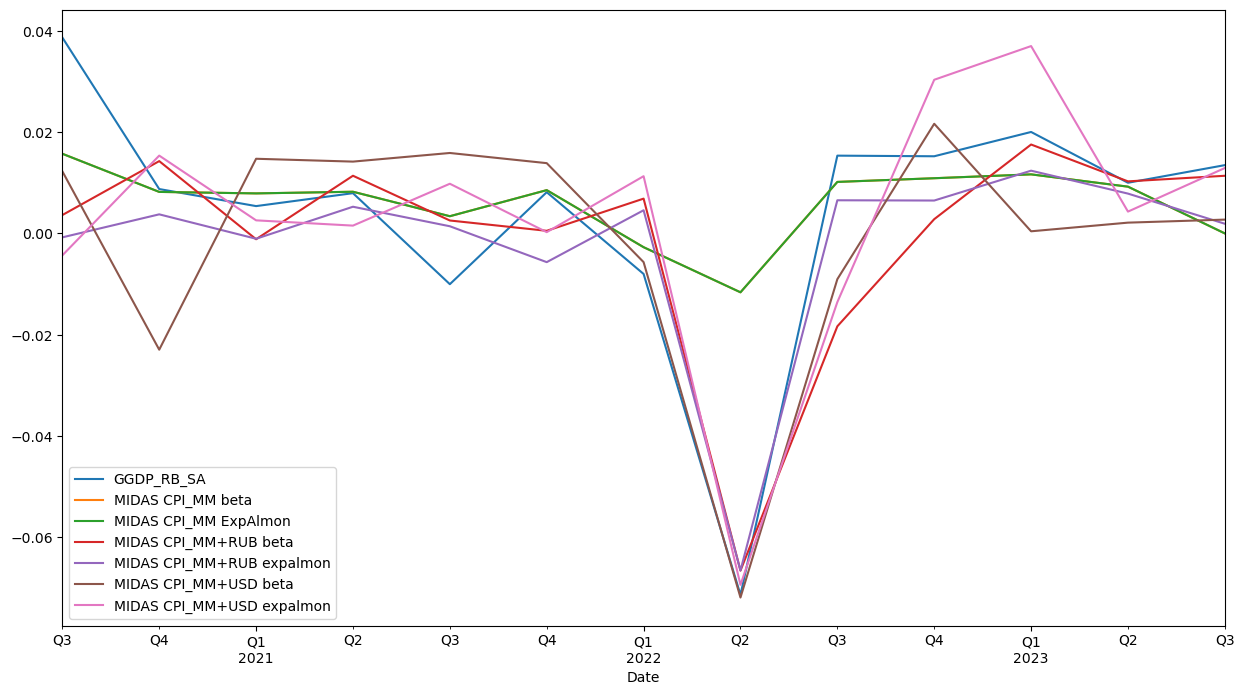
\includegraphics[scale=0.35]{../TeX/images/img06}
		\caption{Графики ретроспективных прогнозов по 12 последним точкам моделей MIDAS регрессии}
		\label{fig:img06}
	\end{figure}
\end{frame}

%--------------------------------------------------------------------------

\begin{frame}
	{Оценки точности построенных моделей}
	\begin{table}[h]
		\centering
		\caption{Retrospective Evaluation Metrics}
		\label{tab:evaluation_metrics}
		\begin{tabular}{|c|c|c|c|}
			\hline
			Model & MAE & MAPE & RMSE \\
			\hline
			MIDAS CPI\_MM Beta          & 0.010561 & 0.473983 & 0.018825 \\
			MIDAS CPI\_MM ExpAlmon      & 0.010561 & 0.473978 & 0.018825 \\
			MIDAS CPI\_MM+RUB Beta      & 0.010875 & 0.816500 & 0.015378 \\
			\textbf{MIDAS CPI\_MM+RUB ExpAlmon}  & \textbf{0.010394} & \textbf{0.784645} & \textbf{0.013824} \\
			MIDAS CPI\_MM+USD Beta      & 0.013635 & 1.152350 & 0.016956 \\
			MIDAS CPI\_MM+USD ExpAlmon  & 0.013467 & 0.993322 & 0.017887 \\
			\hline
		\end{tabular}
	\end{table}
	
	\begin{table}[htbp]
		\centering
		\caption{Future Evaluation Metrics}
		\label{tab:evaluation_metrics}
		\begin{tabular}{|c|c|c|c|}
			\hline
			Model & MAE & MAPE & RMSE \\
			\hline
			MIDAS CPI\_MM Beta          & 0.004407 & 0.787724 & 0.004407 \\
			MIDAS CPI\_MM ExpAlmon      & 0.004407 & 0.787740 & 0.004407 \\
			\textbf{MIDAS CPI\_MM+RUB Beta}      & \textbf{0.001626} & \textbf{0.290612} & \textbf{0.006263} \\
			\textbf{MIDAS CPI\_MM+RUB ExpAlmon}  & \textbf{0.001587} & \textbf{0.283747} & \textbf{0.006301} \\
			MIDAS CPI\_MM+USD Beta      & 0.004614 & 0.824704 & 0.012502 \\
			MIDAS CPI\_MM+USD ExpAlmon  & 0.002240 & 0.400436 & 0.005648 \\
			\hline
		\end{tabular}
	\end{table}
\end{frame}

%--------------------------------------------------------------------------

\begin{frame}
	{Сравнение лучшей MIDAS модели с моделями DL и ARDL}
	\begin{figure}
		\centering
		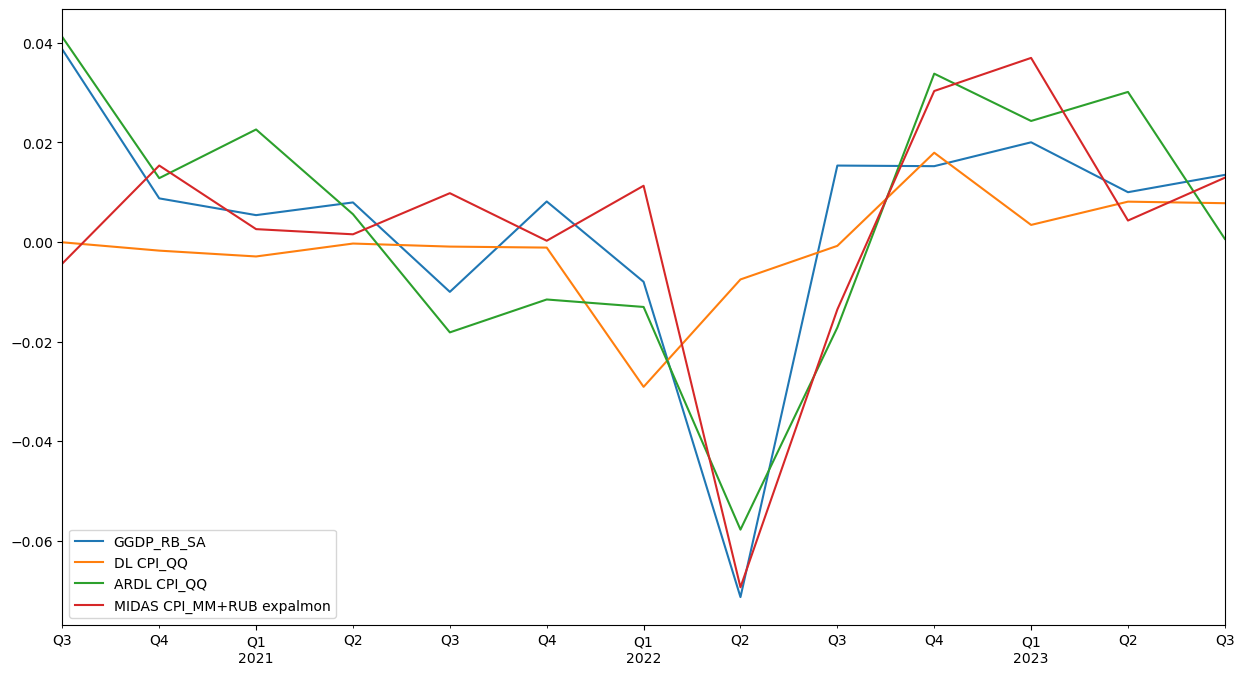
\includegraphics[scale=0.35]{../TeX/images/img09}
		\caption{Графики ретроспективных прогнозов по 12 последним точкам моделей MIDAS, DL и ARDL}
		\label{fig:img09}
	\end{figure}
	
\end{frame}

%--------------------------------------------------------------------------

\begin{frame}
	{Оценка точности моделей MIDAS, DL и ARDL}
	\begin{table}[htbp]
		\centering
		\caption{Evaluation Metrics}
		\label{tab:evaluation_metrics}
		\begin{tabular}{|c|c|c|c|}
			\hline
			Model & MAE & MAPE & RMSE \\
			\hline
			MIDAS CPI\_MM+RUB ExpAlmon & 0.013467 & 0.993322 & 0.017887 \\
			DL CPI\_QQ                 & 0.016318 & 1.001932 & 0.023231 \\
			ARDL CPI\_QQ               & 0.012386 & 1.122417 & 0.015147 \\
			\hline
		\end{tabular}
	\end{table}
\end{frame}

%--------------------------------------------------------------------------

\begin{frame}
	{Заключение}
	Основные результаты работы:
	\begin{itemize}
		\item были математически определены и рассмотрены модели для работы по данным разной частоты;
		\item были исследованы статистические свойства временных рядов ВВП, ИПЦ и курсов валют;
		\item были построены модели MIDAS регрессии и модели с распределенным запаздыванием;
		\item была проведена оценка точности ретроспективных и будущих прогнозов для моделей MIDAS регрессии.
	\end{itemize} 
\end{frame}

%--------------------------------------------------------------------------

\begin{frame}
	{Используемые источники}
	\begin{enumerate}
	\item Foroni, C. A survey of econometric methods for mixed frequency data / C. Foroni, M. Marcellino // Working Paper 2013/06, Norges Bank.
	\item Ghysels, E., Santa-Clara P., Valkanov R. 2002. The MIDAS touch: Mixed data sampling regression models, Working paper, UNC and UCLA.
	\item Макеева, Н.М., Наукастинг элементов использования ВВП России / Н.М. Макеева, И.П. Станкевич // Статья 2022/10, Экономический журнал ВШЭ.
	\item Foroni, C. Unrestricted Mixed Data Sampling (U-MIDAS): MIDAS Regressions With Unrestricted Lag Polynomials / C. Foroni, M. Marcellino, C. Schumacher // Discussion paper 2015, Deutsche Bundesbank.
	\item Станкевич И.П. Сравнение методов наукастинга макроэкономических индикаторов на примере российского ВВП // Прикладная эконометрика 2020. С. 113–127.
	\item Харин, Ю. С. Теория вероятностей, математическая и прикладная статистика / Ю. С. Харин, Н. М. Зуев, Е. Е. Жук // Минск : БГУ, 2011. 
	\end{enumerate}
\end{frame}

\end{document} 